%%%%%%%%%%%%%%%%%%%%%%%%%%%%%%%%%%%%%%%%%%%%%%%%%%%%%%%%%%%%%%%%%%%%%%%%
% Plantilla TFG/TFM
% Escuela Politécnica Superior de la Universidad de Alicante
% Realizado por: Jose Manuel Requena Plens
% Contacto: info@jmrplens.com / Telegram:@jmrplens
%%%%%%%%%%%%%%%%%%%%%%%%%%%%%%%%%%%%%%%%%%%%%%%%%%%%%%%%%%%%%%%%%%%%%%%%

\chapter{Metodología}
\label{metodologia}

\section{Historias de usuario}
Para la gestión ágil de este proyecto, comenzaremos a describir historias de usuario. Siguiendo una estructura sistemática para reflejar las necesidades de los usuarios que se traducen en requisitos funcionales para el sistema que influirán en el diseño y desarrollo de la plataforma.

%-------------------------------------------------------------------
\begin{tcolorbox}[title=Historia de Usuario 1: Añadir KPIs a la pantalla de estadísticas]
\textbf{Como} \textit{Entrenador/a},\\
\textbf{Quiero} Poder añadir y quitar KPIs de la pantalla de estadísticas según sea necesario,\\
\textbf{Para que} Enfocarme en medir y visualizar solo los KPIs específicos que necesito, facilitando la toma de decisiones rápidas y efectivas para mejorar el rendimiento del equipo.
\end{tcolorbox}

\subparagraph{Descripción}
La pantalla para evaluar los indicadores de rendimiento debe mostrar a la vez tantos como el entrenador necesite al mismo tiempo, así como eliminar de la vista aquellos que ya no son relevantes en ese momento.

\subparagraph{Criterios de Aceptación}
\begin{itemize}
    \item El entrenador debe poder acceder a una interfaz de usuario para ver los KPIs.
    \item La aplicación debe recomendar algunos KPIs predefinidos en caso de que haya menos de 5 en la pantalla.
    \item El entrenador debe poder borrar todos los indicadores de una sola vez y limpiar la vista.
\end{itemize}

%-------------------------------------------------------------------
\begin{tcolorbox}[title=Historia de Usuario 2: Creación de nuevos KPIs]
\textbf{Como} \textit{Entrenador/a},\\
\textbf{Quiero} Poder crear y eliminar nuevos indicadores de rendimiento con los datos almacenados en la base de datos,\\
\textbf{Para que} Explotar todos los datos recopilados de una manera eficiente para ver las fortalezas y debilidades del equipo.
\end{tcolorbox}

\subparagraph{Descripción}
Después de cada partido o entrenamiento, los datos comunicados por el entrenador serán almacenados en una base de datos. A partir de esos datos y con una fórmula general, el entrenador debe poder elegir dos datos y crear un nuevo indicador de rendimiento para ser evaluado.

\subparagraph{Criterios de Aceptación}
\begin{itemize}
    \item El entrenador debe poder acceder a una interfaz de usuario para crear los KPIs.
    \item En la interfaz se debe poder definir el nuevo nombre del indicador, descripción y los datos que involucra.
    \item La aplicación no debe permitir nombres repetidos de indicadores.
    \item La aplicación no debe permitir que dos indicadores involucren los mismos datos de la misma forma.
    \item El indicador debe poder asignarse a jugadores o equipos.
\end{itemize}

%-------------------------------------------------------------------
\begin{tcolorbox}[title=Historia de Usuario 3: Edición de KPIs]
\textbf{Como} \textit{Entrenador/a},\\
\textbf{Quiero} Poder editar los indicadores de rendimiento ya sea por su nombre o por sus parámetros,\\
\textbf{Para que} Cambiar los indicadores según el progreso que necesiten mis entrenamientos.
\end{tcolorbox}

\subparagraph{Descripción}
Una vez haya definido al menos un KPI, el entrenador debe ser capaz de editar el nombre, atributos y descripción del indicador. Este cambio puede ser debido ya sea por el cambio de opinión del entrenador del entrenador, o por una necesidad de utilizar ese nombre o parámetros para otra perspectiva en las sesiones de entrenamiento.

\subparagraph{Criterios de Aceptación}
\begin{itemize}
    \item El entrenador debe poder seleccionar un KPI existente en la interfaz para editarlo.
    \item La interfaz de edición debe poder permitir editar el nombre, parámetros del KPI o jugadores y equipo a los cuales esté asignado este indicador.
    \item Los cambios deben de ser en cascada, reflejando la modificación en todas las vistas en las que el KPI esté implicado.
    \item Se debe permitir cancelar la edición si el usuario cambia de idea.
\end{itemize}

%-------------------------------------------------------------------
\begin{tcolorbox}[title=Historia de Usuario 4: Ver estadísticas]
\textbf{Como} \textit{Jugador/a},\\
\textbf{Quiero} Poder ver un listado de todas mis estadísticas y mis indicadores de rendimiento,\\
\textbf{Para que} Poder fijarme en mis puntos débiles e intentar mejorarlos según me dicte el entrenador.
\end{tcolorbox}

\subparagraph{Descripción}
Cada jugador debe poder acceder a una interfaz donde se muestren todos los indicadores que el entrenador ha asociado a ese jugador en concreto, también debería ver una gráfica sobre el progreso y la evolución de sus indicadores. Así se podría fomentar la auto-crítica por parte del jugador.

\subparagraph{Criterios de Aceptación}
\begin{itemize}
    \item Los jugadores deben poder acceder a un menú propio donde se muestren sus datos.
    \item El menú debe incluir gráficas con marcas temporales.
    \item Se de poder filtrar por rango de fechas, seleccionar estadísticas para que solo se muestren esas y por tipos de estadísticas.
\end{itemize}

%-------------------------------------------------------------------
\begin{tcolorbox}[title=Historia de Usuario 5: Ver progreso de los jugadores]
\textbf{Como} \textit{Entrenador/a},\\
\textbf{Quiero} Poder generar un informe gráfico que muestre la evolución de los KPIs asociados a jugadores,\\
\textbf{Para que} Poder evaluar a mis jugadores y darles las indicaciones adecuadas para maximizar el margen de mejora de mi equipo.
\end{tcolorbox}

\subparagraph{Descripción}
El entrenador es el primer responsable del equipo y de él depende que los jugadores mejoren y exploten sus capacidades lo máximo posible. Es por ello que debe de ser capaz de generar en la plataforma un informe, ya sea individual de cada jugador o grupal, sobre la evolución de las estadísticas de éstos.

\subparagraph{Criterios de Aceptación}
\begin{itemize}
    \item Los entrenadores deben poder seleccionar uno o varios jugadores junto con uno o varios KPIs para generar el informe.
    \item El menú debe incluir gráficas con marcas temporales.
    \item La plataforma debe de ser capaz de detectar una mejora o un empeoramiento de las habilidades del jugador.
\end{itemize}


%-------------------------------------------------------------------
\begin{tcolorbox}[title=Historia de Usuario 6: Alinear jugadores del Equipo]
\textbf{Como} \textit{Entrenador/a},\\
\textbf{Quiero} Poder crear nuevas alineaciones con mis jugadores del equipo,\\
\textbf{Para que} Plantear tácticas, posicionar jugadores y descubrir y fortalecer las buenas posiciones para mis jugadores.
\end{tcolorbox}

\subparagraph{Descripción}
Entender las posiciones de los jugadores es una tarea clave para el entrenador, por ello ha de ser capaz de poder crear nuevas alineaciones con sus jugadores para poder entenderlos a la perfección.

\subparagraph{Criterios de Aceptación}
\begin{itemize}
    \item Los entrenadores deben poder acceder a un menú dentro de la vista del equipo para la creación de alineaciones.
    \item Un jugador no puede aparecer dos veces en la misma alineación.
    \item En la vista de la alineación, se debe poder editar y eliminar toda la alineación.
    \item Se dispondrá de alineaciones comunes predefinidas, con la posibilidad del entrenador de crear las suyas propias.
    \item No podrán existir dos alineaciones exactamente iguales (mismos jugadores en la misma posición).
\end{itemize}

%-------------------------------------------------------------------
\begin{tcolorbox}[title=Historia de Usuario 7: Análisis y Reportes Detallados]
\textbf{Como} \textit{Entrenador/a},\\
\textbf{Quiero} Generar reportes detallados de rendimiento por jugador y por equipo,\\
\textbf{Para que} Tener un seguimiento preciso del progreso a lo largo del tiempo.
\end{tcolorbox}

\subparagraph{Descripción}
Más allá de un visualizado de estadísticas y gráficas, el entrenador debe se capaz de generar informes completos sobre el desarrollo de los jugadores.

\subparagraph{Criterios de Aceptación}
\begin{itemize}
    \item Para generar los informes, se debe poder seleccionar métricas específicas.
    \item Los informes pueden ser exportados en formatos PDF, Excel o CSV.
    \item Los informes deben contener gráficas de tendencias y otras comparativas.
\end{itemize}

%-------------------------------------------------------------------
\begin{tcolorbox}[title=Historia de Usuario 8: Sistema de comunicación]
\textbf{Como} \textit{Entrenador/a o jugador/a},\\
\textbf{Quiero} Poder comunicarme con mis jugadores/entrenador,\\
\textbf{Para que} favorecer la comunicación y mejorar el ambiente del equipo.
\end{tcolorbox}

\subparagraph{Descripción}
Además del seguimiento de estadísticas, si ocurren acontecimientos que requieran de una conversación entre el entrenador y el jugador se debería contar con un sistema simple de mensajería. Con este pequeño sistema dentro de la plataforma, es posible fomentar un ambiente de equipo positivo siguiendo las palabras de Sir Alex Ferguson en \cite{TheGuardian} .

\subparagraph{Criterios de Aceptación}
\begin{itemize}
    \item Debe de exisitr una interfaz dedicada a la mensajería.
    \item Las conversaciones permanecerán almacenadas hasta que el usuario decida borrarlas.
    \item Se debe poder iniciar y borrar conversaciones desde un menú.
    \item No podrán existir dos chats con la misma persona.
\end{itemize}


%-------------------------------------------------------------------
\begin{tcolorbox}[title=Historia de Usuario 9: Acceso a roles de usuario]
\textbf{Como} \textit{Usuario},\\
\textbf{Quiero} Poder acceder a los datos a los que tenga acceso,\\
\textbf{Para que} Realizar el seguimiento siendo o el mismo jugador o el tutor legal de éste.
\end{tcolorbox}

\subparagraph{Descripción}
Los padres y tutores también tienen derecho a ver el seguimiento de sus hijos/as, por ello es considerable añadir roles de usuario para que cada persona responsable pueda ver sus propios datos.

\subparagraph{Criterios de Aceptación}
\begin{itemize}
    \item La plataforma debe tener definidos claramente los roles de "Entrenador", "Jugador", "Padre/Tutor" y "Administrador".
    \item Cada rol debe poder acceder únicamente a los datos que le corresponden según las definiciones de permisos.
    \item Debe existir un sistema de autenticación para los usuarios.
    \item La plataforma debe cumplir con las normativas locales e internacionales de protección de datos
\end{itemize}

%-------------------------------------------------------------------
\begin{tcolorbox}[title=Historia de Usuario 10: Intervalos Estadísticos para el menú]
\textbf{Como} \textit{Entrenador/a},\\
\textbf{Quiero} Poder alternar el intervalo de tiempo en el que se mide la estadística,\\
\textbf{Para que} Tener un mejor control de la evolución de mis equipos durante el periodo de tiempo que estime útil.
\end{tcolorbox}

\subparagraph{Descripción}
Para que el seguimiento de los resultados sea lo mas eficaz y eficiente posible, el entrenador debe poder alternar el intervalo de tiempo en el que se miden los resultados para su propio interés. Si quiere ver resultados a corto plazo, podrá ver la evolución partido a partido, si quiere resultados a largo plazo, oidrá verla mensual o trimestralmente.

\subparagraph{Criterios de Aceptación}
\begin{itemize}
    \item La plataforma tendrá un menú superior para alternar el intervalo.
    \item Cuando se alterna la opción, todas las vistas serán actualizadas para mostrar la evolución de los jugadores dentro del intervalo seleccionado.
\end{itemize}

%Para Añadir:
%- Creación de secciones para los KPIs
%- Intervalos Estadísticos para el menú
%- DAFO para la ficha de jugadores

\section{Elección de las tecnologías y lenguajes de programación}
A continuación, detallamos las razones específicas para la elección de las siguientes herramientas como componentes clave del desarrollo.

\subsection{Git}
Git es un software de control de versiones gratis y de código abierto, funciona como un rastreador de contenido permitiendo a los desarrolladores revertir y regresar a una versión anterior de su código. Con Git, cada desarrollador tiene una copia completa del repositorio, lo que permite trabajar sin conexión y realizar operaciones localmente. Además, Git soporta la creación de ramas para trabajar en nuevas características o correcciones de errores de manera independiente, que luego pueden fusionarse en la rama principal. Su uso de algoritmos de hashing garantiza la integridad de los datos, y su rendimiento superior permite manejar grandes cantidades de datos y cambios de manera eficiente.


\subsection{Visual Studio Code}


\subsection{VueJS}

\subsubsection{Dependencias}
\subparagraph{Iconify}
%https://es.linux-console.net/?p=28105
%https://iconify.design/getting-started/

Iconify es un proyecto de código abierto que proporciona una forma sencillade utilizar iconos dentro de las aplicaciones Vue. El paquete que ofrece, \textbf{@iconify/vue}, permite agregar y personalizar rápidamente iconos en nuestro proyecto. Para instalarlo, ejecutaremos el comando de instalación:

\begin{lstlisting}[style=Consola, caption={Instalación del paquete iconify},label=Consola_code]
	npm install --save-dev @iconify/vue
\end{lstlisting}

Para agregar los iconos que ofrece Iconify debemos importar el componente Icon del paquete en nuestros componentes de Vue. Lo haremos con el siguiente fragmento de código:

\begin{lstlisting}[style=PHP-color, caption={Importar el componente Icon en Vue},label=PHP-color_code]
	<script setup>
		import { Icon } from '@iconify/vue'
	</script>
\end{lstlisting}

Para agregar iconos debemos buscar los que queramos en la página web de Iconify en \citep{iconos-iconify}. Una vez hayamos elegido el estilo del icono, podemos copiar el código del componente en la página web, por ejemplo:

\begin{lstlisting}[style=PHP-color, caption={Código para agregar un icono a la página},label=PHP-color_code]
	<template>
		<Icon icon="streamline:graph-dot-solid" />
	</template>
\end{lstlisting}

Dando como resultado:
\begin{figure}[H]
    \centering
    
\includegraphics[width=3cm]{archivos/tfg_jorge/icoco_grafico_iconify}
    \caption{Icono de gráfico importado desde la biblioteca de Iconify}\label{sistemass2}
\end{figure}

\subparagraph{ViteJS}
ViteJS es una herramienta de construcción de frontend que ofrece una experiencia de desarrollo moderna, rápida y eficiente para proyectos web.
Gracias a su recarga instantánea podemos mejorar considerablemente la productividad a medida que desarrollamos el proyecto. Nuestro proyecto principal de Vue lo crearemos con esta herramienta:

\begin{lstlisting}[style=Consola, caption={Instalación del paquete iconify},label=Consola_code]
	npm init @vitejs/app
\end{lstlisting}

\subparagraph{ChartJS}
Una biblioteca de JavaScript que permite crear gráficos interactivos y visualizaciones de datos en aplicaciones web. Es fácil de usar y compatible con múltiples tipos de gráficos, como barras, líneas, etc. Gracias a su sencillez para integrarla en nuestro proyecto de Vue podremos usarla con total normalidad.

Para usarla, crearemos un componente para la creación de una gráfica que podremos usar en todas las vistas que queramos:

\begin{lstlisting}[style=PHP-color, caption={Código para agregar un icono a la página},label=PHP-color_code]
<template>
  <div class="chart-container">
    <canvas :id="chartId"></canvas>
  </div>
</template>


<script>
import Chart from 'chart.js/auto';

export default {
  name: 'KpiChart',
  props: {
    chartData: {
      type: Array,
      required: true
    },
    chartId: {
      type: String,
      required: true
    },
    chartName: {
      type: String,
      required: true
    }
  },
  mounted() {

    try{
      const ctx = document.getElementById(this.chartId);
      if (this.chartData && this.chartData.length > 0) {
        new Chart(ctx, {
          type: 'line',
          data: {
            labels: this.chartData.map(row => row.time),
            datasets: [
              {
                label: this.chartName,
                data: this.chartData.map(row => row.score)
              }
            ]
          },
          options: {
            animation: {
              duration: 1500, // milisegundos
              easing: 'easeOutCubic', // Tipo de animación
              onProgress(animation) {
                const chartInstance = animation.chart;
                const ctx = chartInstance.ctx;
                const dataset = chartInstance.data.datasets[0];
                const meta = chartInstance.getDatasetMeta(0);
                meta.data.forEach((bar, index) => {
                  const data = dataset.data[index];
                  ctx.fillText(data, bar.x, bar.y - 5);
                });
              },
              onComplete(animation) {
                const chartInstance = animation.chart;
                const ctx = chartInstance.ctx;
                const dataset = chartInstance.data.datasets[0];
                const meta = chartInstance.getDatasetMeta(0);
                meta.data.forEach((bar, index) => {
                  const data = dataset.data[index];
                  ctx.fillText(data, bar.x, bar.y - 5);
                });
              }
            },
          }
        });
      } else {
        console.error('No hay datos para la grafica');
      }
    }
    catch(error){
      console.error("Error:",error)
    }
  }
};
</script>
\end{lstlisting}

Como resultado de una de nuestras gráficas:
\begin{figure}[H]
    \centering
    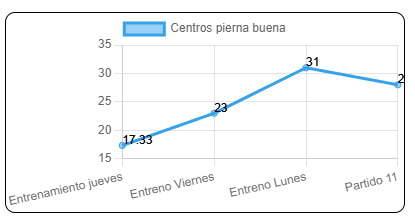
\includegraphics[width=6cm]{archivos/tfg_jorge/chartjs_ejemplo}
    \caption{Gráfico generado con ChartJS}
    \label{sistemass2}
\end{figure}

\subparagraph{Vue-router}

\subparagraph{Vuex}


\subsection{MySQL Server}

\subsection{Framework DAO}
Cambiar en database.js \lstinline|require("mysql")| por \lstinline|mysql2|, compatible con el método \lstinline|auth_caching_sha2_password|, el que viene en MySQL Server 8.4.

